\let\negmedspace\undefined
\let\negthickspace\undefined
\documentclass[a4,12pt,onecolumn]{IEEEtran}
\usepackage{amsmath,amssymb,amsfonts,amsthm}
\usepackage{algorithmic}
\usepackage{graphicx}
\usepackage{textcomp}
\usepackage{xcolor}
\usepackage{txfonts}
\usepackage{listings}
\usepackage{enumitem}
\usepackage{mathtools}
\usepackage{gensymb}
\usepackage[breaklinks=true]{hyperref}
\usepackage{tkz-euclide}
\usepackage{listings}
\usepackage{gvv}
\DeclareMathOperator*{\Res}{Res}
\renewcommand\thesection{\arabic{section}}
\renewcommand\thesubsection{\thesection.\arabic{subsection}}
\renewcommand\thesubsubsection{\thesubsection.\arabic{subsubsection}}
\renewcommand\thesectiondis{\arabic{section}}
\renewcommand\thesubsectiondis{\thesectiondis.\arabic{subsection}}
\renewcommand\thesubsubsectiondis{\thesubsectiondis.\arabic{subsubsection}}
\hyphenation{op-tical net-works semi-conduc-tor}
\def\inputGnumericTable{}                                
\lstset{
frame=single, 
breaklines=true,
columns=fullflexible
}
\begin{document}
\newtheorem{theorem}{Theorem}[section]
\newtheorem{problem}{Problem}
\newtheorem{proposition}{Proposition}[section]
\newtheorem{lemma}{Lemma}[section]
\newtheorem{corollary}[theorem]{Corollary}
\newtheorem{example}{Example}[section]
\newtheorem{definition}[problem]{Definition}
\newcommand{\BEQA}{\begin{eqnarray}}
\newcommand{\EEQA}{\end{eqnarray}}
\newcommand{\define}{\stackrel{\triangle}{=}}
\bibliographystyle{IEEEtran}
\providecommand{\mbf}{\mathbf}
\providecommand{\pr}[1]{\ensuremath{\Pr\left(#1\right)}}
\providecommand{\qfunc}[1]{\ensuremath{Q\left(#1\right)}}
\providecommand{\sbrak}[1]{\ensuremath{{}\left[#1\right]}}
\providecommand{\lsbrak}[1]{\ensuremath{{}\left[#1\right.}}
\providecommand{\rsbrak}[1]{\ensuremath{{}\left.#1\right]}}
\providecommand{\brak}[1]{\ensuremath{\left(#1\right)}}
\providecommand{\lbrak}[1]{\ensuremath{\left(#1\right.}}
\providecommand{\rbrak}[1]{\ensuremath{\left.#1\right)}}
\providecommand{\cbrak}[1]{\ensuremath{\left\{#1\right\}}}
\providecommand{\lcbrak}[1]{\ensuremath{\left\{#1\right.}}
\providecommand{\rcbrak}[1]{\ensuremath{\left.#1\right\}}}
\theoremstyle{remark}
\newtheorem{rem}{Remark}
\newcommand{\sgn}{\mathop{\mathrm{sgn}}}
\providecommand{\res}[1]{\Res\displaylimits_{#1}} 
\providecommand{\mtx}[1]{\mathbf{#1}}
\providecommand{\fourier}{\overset{\mathcal{F}}{ \rightleftharpoons}}
\providecommand{\system}{\overset{\mathcal{H}}{ \longleftrightarrow}}
\newcommand{\solution}{\noindent \textbf{Solution: }}
\newcommand{\cosec}{\,\text{cosec}\,}
\providecommand{\dec}[2]{\ensuremath{\overset{#1}{\underset{#2}{\gtrless}}}}
\newcommand{\myvec}[1]{\ensuremath{\begin{pmatrix}#1\end{pmatrix}}}
\newcommand{\mydet}[1]{\ensuremath{\begin{vmatrix}#1\end{vmatrix}}}
\let\vec\mathbf
\title{
\Huge\textbf{Discrete Assignment}\\
\Huge\textbf{EE1205} Signals and Systems\\
}
\large\author{Kurre Vinay\\EE23BTECH11036}
\maketitle
\bigskip
\renewcommand{\thefigure}{\theenumi}
\renewcommand{\thetable}{\theenumi}
\textbf{Question 11.9.3.8:}
Find the sum to indicated number of term in each of the geometric progressions in $\sqrt{7} ,\sqrt{21} , 3\sqrt{7}, ....n$ terms\\
\solution
 \begin{center}
\begin{tabular}{|c|c|c|}
   \hline
   variable&value&description  \\
   \hline
   $x(0)$ & $ \sqrt{7} $& first term of the geometric progession\\
   \hline
   $r$ & $\sqrt{3}$ & common ratio of the geometeric progression\\
   \hline
   $x(n)$ & $\sqrt{7(3^{n})}u\brak{n}$& $n^{th}$ term of the geometric progession\\
   \hline
   $y(n)$ &$\frac{x(0)(r^{n+1}-1)}{r-1}u\brak{n}$ &Sum of the n term of the geometric progression\\
   \hline 
   
\end{tabular}
\\\\ \caption{\large{Table : Input parameters}}\\
\end{center}
\begin{center}
\begin{align}
X\brak{z} &= x\brak{0}\brak{\frac{1}{1-rz^{-1}}}, \quad{|rz^{-1}|<1}\\
y\brak{n} &= x\brak{n}*u\brak{n}\\
Y\brak{z} &= X\brak{z}U\brak{z}\\
&=\sqrt{7}\brak{\frac{1}{1-\sqrt{3}z^{-1}}}\brak{\frac{1}{1-z^{-1}}} ,\quad{|z|>\sqrt{3}}\\
&=\brak{\frac{\sqrt{7}}{\sqrt{3}-1}}\brak{\brak{\frac{\sqrt{3}}{1-\sqrt{3}z^{-1}}}-\brak{\frac{1}{1-z^{-1}}}}\\
\frac{1}{1-rz^{-1}} &$$\xleftrightarrow{\mathcal{Z}^{-1}} $$ r^nu(n), \quad{|z|>r}\\
y\brak{n} &= \sqrt{7}\brak{\frac{\sqrt{3}^{n+1}-1}{\sqrt{3}-1}}u(n) , \quad{|z|>\sqrt{3}}\end{align}

\end{center}
\begin{figure}[ht!]
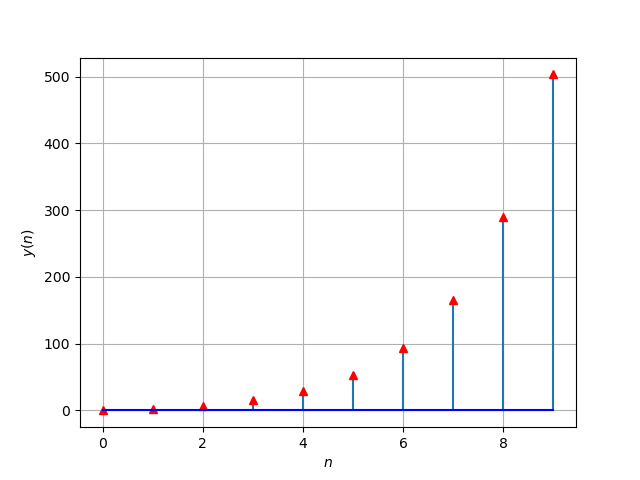
\includegraphics[width=\columnwidth]{fig/fig1.png}
\caption{\large{STEM PLOT OF $y\brak{n}$}}
\end{figure}
\end{document}
